%
% Transportation Research Board conference paper template
% version 1.1
% 
% David R. Pritchard, http://davidpritchard.org
%   1.0 - Mar. 2009
%   1.1 - Sep. 2011, fixes for captions
%   2.0 - Mar. 2012, Reorganized title page incl. automatic counters

% PAGE LAYOUT
%------------------------------------------

% Custom paper settings...
\documentclass[titlepage,oneside,12pt]{article}

\oddsidemargin 0.0in
\topmargin -0.5in
\headheight 0.3in
\headsep 0.2in
\textwidth 6.5in
\textheight 9.0in
\setlength{\parindent}{0.5in}

% PAGE HEADER
%------------------------------------------
% Adjust the header text below (INSERT AUTHORS HERE)
\oddsidemargin 0.0in
\usepackage[tiny,rm]{titlesec}
\newpagestyle{trbstyle}{
	\sethead{Pritchard and Macfarlane}{}{\thepage}
}
\pagestyle{trbstyle}

% HEADINGS
%------------------------------------------
\renewcommand*{\refname}{\uppercase{References}}
\titleformat{\section}{\bfseries}{}{0pt}{\uppercase}
\titlespacing*{\section}{0pt}{12pt}{*0}
\titleformat{\subsection}{\bfseries}{}{0pt}{}
\titlespacing*{\subsection}{0pt}{12pt}{*0}
\titleformat{\subsubsection}{\itshape}{}{0pt}{}
\titlespacing*{\subsubsection}{0pt}{12pt}{*0}

% LISTS
%------------------------------------------
% Adjust lists a little. Not quite perfectly fitting TRB style, but vaguely
% close at least.
\usepackage{enumitem}
\setlist[1]{labelindent=0.5in,leftmargin=*}
\setlist[2]{labelindent=0in,leftmargin=*}

% CAPTIONS
%------------------------------------------
% Get the captions right. Authors must still be careful to use "Title Case"
% for table captions, and "Sentence case." for figure captions.
\usepackage{ccaption}
\usepackage{amsmath}
\makeatletter
\renewcommand{\fnum@figure}{\textbf{FIGURE~\thefigure} }
\renewcommand{\fnum@table}{\textbf{TABLE~\thetable} }
\makeatother
\captiontitlefont{\bfseries \boldmath}
\captiondelim{\;}
%\precaption{\boldmath}


% CITATIONS
%------------------------------------------
% TRB uses an Author (num) citation style. I haven't found a way to make
% LaTeX/Bibtex do this automatically using the standard \cite macro, but
% this modified \trbcite macro does the trick.

% sort&compress option?
\usepackage[sort,numbers]{natbib}
	\newcommand{\trbcite}[1]{\citeauthor{#1} ({\it \citenum{#1}})}
\setcitestyle{round}


% LINE NUMBERING
%------------------------------------------
% TRB likes line numbers on drafts to help reviewers refer to parts of the
% document. The numbering is activated with the \linenumbers command immediately
% after \begin{document} You may need to install the lineno  package from CTAN.
\usepackage[pagewise]{lineno}
	\renewcommand\linenumberfont{\normalfont\small}


% COUNTERS
%------------------------------------------
% TRB requires the total number of words, figures, and tables to be displayed on
% the title page. This is possible under the totcount package on CTAN.
\usepackage{totcount}
	\regtotcounter{table} 	%count tables
	\regtotcounter{figure} 	%count figures

\newcommand\wordcount{
    \immediate\write18{texcount -sum -1 \jobname.tex > 'count.txt'} \input{count.txt} }

% FONTS
%------------------------------------------
% Times for text and math
\usepackage{mathptmx}


% Some pdf conversion tricks? Unsure.
\usepackage[T1]{fontenc}
\usepackage{textcomp}
% Fonts will be broken by Sweave without this option
\usepackage[noae]{Sweave}


% OTHER PACKAGES
%------------------------------------------
% Add any additional \usepackage declarations here.

\usepackage{graphicx}


% TITLEPAGE
%-----------------------------------------
\begin{document}

	\pagewiselinenumbers % comment out for final manuscript
	\thispagestyle{empty}

\begin{titlepage}
\begin{flushleft}

% Title
{\LARGE \bfseries A \LaTeX\ Template for Papers Submitted to the Transportation
Research Board}\\[1cm]

David Pritchard \\
davidpritchard.org\\[0.5cm]

Gregory S. Macfarlane\\
Georgia Institute of Technology \\
790 Atlantic Drive \\
Atlanta, GA 30332-0335 \\
gregmacfarlane@gatech.edu\\[1cm]

%\wordcount words + \total{figure} figures + \total{table} tables

\today
\end{flushleft}
\end{titlepage}


\newpage

\thispagestyle{empty}
\section{Abstract}
The Transportation Research Board has unique and seemingly arbitrary
requirements for manuscripts submitted for review. These requirements make it
difficult to write the manuscripts quickly, and no existing \LaTeX\ style comes
close to fooling the guidelines. This represents an initial effort at creating a
template to meet the requirements of TRB authors using \LaTeX, Sweave, or other
literate programming software.

\newpage

\section{Introduction}
The \trbcite{TRBGuide} has unique and somewhat arbitrary requirements
for papers submitted for review and publication. While the initial submission is
required to be in PDF format, submissions for publication in Transportation
Research Record must be in Microsoft Office format. On top of this, the
manuscripts must be line-numbered, captions are bolded and employ atypical
punctuation, and the references must be numbered when cited and then printed in
order.

It is assumed that the readers of this document have some significant level of
experience in \LaTeX and \verb1bibtex1. As use of literate programming becomes more
widespread in engineering and planning, it is possible that this template may
need to be made more robust.

\subsection{History}
David Pritchard posted the original versions of this template in 2009 and
updated it in 2011, soon after TRB began allowing PDF submissions. Gregory
Macfarlane made significant adaptations to it in March 2012, allowing for Sweave
integration and automatic word and table counts.



\section{Features}
The template has a number of features that enable quick and painless manuscript
authoring.

\subsection{Title Page}
The standard \LaTeX\ \verb1\maketitle1 command is not very versatile, so we have
replaced it with a \verb1titlepage1 environment. This means that the writers
will be required to manually enter spacings based on the number of contributors,
but the current settings (0.5 cm between authors, 1 cm before and after them)
seems to work well. 

Near the bottom of the title page, TRB requires a count of the manuscript's
words, figures, and tables. This template creates these counts automatically.
The figure and table counts are simply pulled from the \LaTeX\ counters using the
\verb1totcount1 package. The word count feature is not as simple, as it
utilizes a call to the system command \verb1texcount1. Thus to compile the
document writers must enable \verb#\write18# in their \verb1pdflatex1 call.

\subsection{Page Layout}
The document has 1 inch margins as required, with the author's names in the left
heading and the page number in the right. The authors heading will need to be
edited by the writers; automating this from the title page command is not
currently possible. Paragraphs leading sections and subsections are not
indented, while all subsequent paragraphs in that section are. Section types are
defined as outlined by the \trbcite{TRBGuide}


The document is single-spaced in 12 point Times font. Times New Roman is a
proprietary font and is therefore not available by installation in open-source
software. While the differences between Times variants are negligible, Times New
Roman itself can be used in Mac OSX by compiling under \verb1xelatex1.


\subsubsection{Line Numbers}
Manuscript line numbering is implemented using the \verb1lineno1 package. There
are options to change the font style and type, but the current settings work
well. Note that the line numbers refresh each page, and that blank lines do not
receive a number.

\section{Captions}
Figure \ref{fig:trial} shows a Gumbel distribution as an example of captioning.
As demonstrated, figure captions ought to be sentence capitalized, bolded, and
can be somwhat longer than in other journals.

Table captions are somewhat different, requiring initial capitals and are more of a
title. An example of this is given in Table \ref{tab:versions}, showing the
history of this template.

\begin{figure}[t]
	\centering
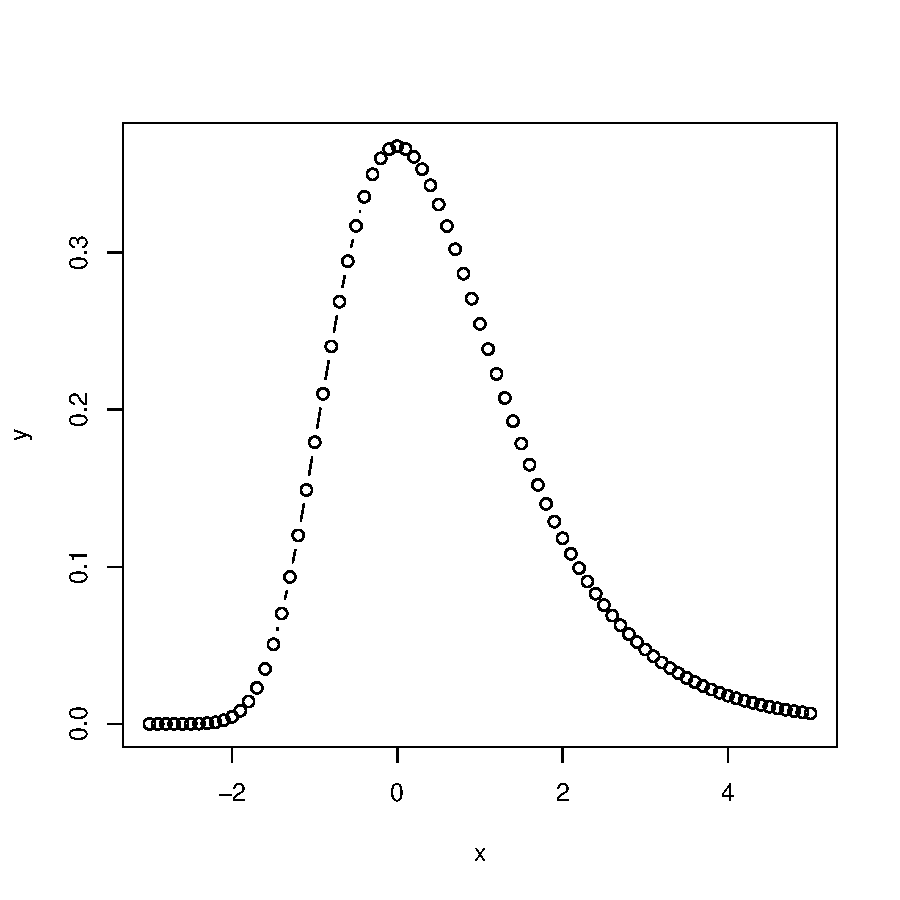
\includegraphics{TRBLaTeX-gumbel}
	\caption{This is a random figure to test the counting functionality on the
title page. It shows a Gumbel distribution with mode 0 and scale 1. The
multinomial logit model assumes that the error terms are distributed identically
and independently following this pattern.}
	\label{fig:trial}
\end{figure}


\begin{table}[t]
	\caption{A History of this Template}
	\label{tab:versions}
\begin{center}
	\begin{tabular}{l l l l}
Version & Date & Author & Contributions \\\hline
1.0 & Sep 2009 & Pritchard & Initial Work \\
1.1 & Mar 2011 & Pritchard & Captions \\
2.0 & Mar 2012 & Macfarlane& Automation, documentation\\\hline
\end{tabular}
\end{center}
\end{table}


\subsection{Bibliography}
The TRB bibliography style is defined in the \verb1trb.bst1 file which should be
in your document folder. A new command is specified, \verb1\trbcite{}1 which
will print the authors and the number of the reference in the order in which it
is supplied. The References section will be appended to the end of the document.

It is very easy to add reference to papers programs written by
\trbcite{Bierlaire2003} and \trbcite{Bierlaire2008} or to papers like those
written by \trbcite{Garrow2009} and \trbcite{Koppelman2005}. You can even go
back and refer to Biog\'eme by \trbcite{Bierlaire2008} a second time.

\section{To Do's}
There is still work to be done on this template. Currently, the word count
feature includes text in the abstract. It would also be cleaner if cited authors
could be separated from their works. This may be possible currently, using the
the \verb1\citeauthor{}1 and \verb1\citenum{}1 commands that are stuck together
into \verb1\trbcite1. 

There may well be other important features in the template that we have not
considered. Ideally, we would make a \verb1trb.sty1 style class that could be
called and we would not have to expose the user to so much \TeX-ese. This could
be forthcoming, but not for this TRB cycle. 


\section{Conclusion}
To make this document from source in a Unix-like OS, issue the following
commands:
\begin{verbatim}
R CMD SWEAVE 'document.rnw'
pdflatex --shell-escape document.tex
bibtex document
pdflatex --shell-escape document.tex
pdflatex --shell-escape document.tex
\end{verbatim}
The \verb1--shell-escape1 option is required to access the command line for the
word count. Normally this feature is disabled because it is a route of entry for
malicious software. Mr.\ Macfarlane promises that there is no such debilitating
code in this document, and he encourages you to examine any scripts for
suspicious code before permitting \verb1pdflatex1 from accessing your system.

\bibliographystyle{trb}
\bibliography{TRBLaTeX}

% End line numbering
\nolinenumbers
\end{document}
